% Created by tikzDevice version 0.12 on 2019-05-23 20:09:48
% !TEX encoding = UTF-8 Unicode
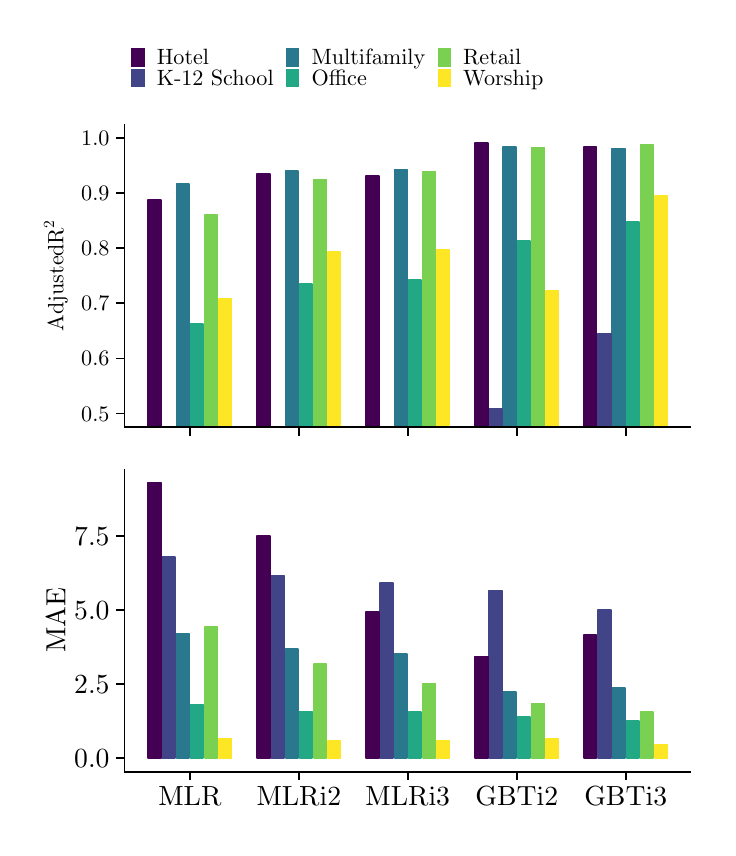
\begin{tikzpicture}[x=1pt,y=1pt]
\definecolor{fillColor}{RGB}{255,255,255}
\path[use as bounding box,fill=fillColor,fill opacity=0.00] (0,0) rectangle (245.72,289.08);
\begin{scope}
\path[clip] (  0.00,135.70) rectangle (245.72,289.08);
\definecolor{drawColor}{RGB}{255,255,255}
\definecolor{fillColor}{RGB}{255,255,255}

\path[draw=drawColor,line width= 0.6pt,line join=round,line cap=round,fill=fillColor] (  0.00,135.70) rectangle (245.72,289.08);
\end{scope}
\begin{scope}
\path[clip] (  0.00,  0.00) rectangle (245.72,135.70);
\definecolor{drawColor}{RGB}{255,255,255}
\definecolor{fillColor}{RGB}{255,255,255}

\path[draw=drawColor,line width= 0.6pt,line join=round,line cap=round,fill=fillColor] (  0.00,  0.00) rectangle (245.72,135.70);
\end{scope}
\begin{scope}
\path[clip] ( 34.98,144.70) rectangle (239.72,254.17);
\definecolor{fillColor}{RGB}{255,255,255}

\path[fill=fillColor] ( 34.98,144.70) rectangle (239.72,254.17);
\definecolor{drawColor}{RGB}{253,231,37}
\definecolor{fillColor}{RGB}{253,231,37}

\path[draw=drawColor,line width= 0.6pt,line join=round,fill=fillColor] ( 69.11, 50.16) rectangle ( 73.70,191.08);
\definecolor{drawColor}{RGB}{122,209,81}
\definecolor{fillColor}{RGB}{122,209,81}

\path[draw=drawColor,line width= 0.6pt,line join=round,fill=fillColor] ( 63.99, 50.16) rectangle ( 68.58,221.33);
\definecolor{drawColor}{RGB}{34,168,132}
\definecolor{fillColor}{RGB}{34,168,132}

\path[draw=drawColor,line width= 0.6pt,line join=round,fill=fillColor] ( 58.87, 50.16) rectangle ( 63.46,181.92);
\definecolor{drawColor}{RGB}{42,120,142}
\definecolor{fillColor}{RGB}{42,120,142}

\path[draw=drawColor,line width= 0.6pt,line join=round,fill=fillColor] ( 53.75, 50.16) rectangle ( 58.34,232.68);
\definecolor{drawColor}{RGB}{65,68,135}
\definecolor{fillColor}{RGB}{65,68,135}

\path[draw=drawColor,line width= 0.6pt,line join=round,fill=fillColor] ( 48.63, 50.16) rectangle ( 53.23,108.88);
\definecolor{drawColor}{RGB}{68,1,84}
\definecolor{fillColor}{RGB}{68,1,84}

\path[draw=drawColor,line width= 0.6pt,line join=round,fill=fillColor] ( 43.51, 50.16) rectangle ( 48.11,226.90);
\definecolor{drawColor}{RGB}{253,231,37}
\definecolor{fillColor}{RGB}{253,231,37}

\path[draw=drawColor,line width= 0.6pt,line join=round,fill=fillColor] (108.48, 50.16) rectangle (113.07,208.00);
\definecolor{drawColor}{RGB}{122,209,81}
\definecolor{fillColor}{RGB}{122,209,81}

\path[draw=drawColor,line width= 0.6pt,line join=round,fill=fillColor] (103.36, 50.16) rectangle (107.95,234.27);
\definecolor{drawColor}{RGB}{34,168,132}
\definecolor{fillColor}{RGB}{34,168,132}

\path[draw=drawColor,line width= 0.6pt,line join=round,fill=fillColor] ( 98.24, 50.16) rectangle (102.83,196.45);
\definecolor{drawColor}{RGB}{42,120,142}
\definecolor{fillColor}{RGB}{42,120,142}

\path[draw=drawColor,line width= 0.6pt,line join=round,fill=fillColor] ( 93.12, 50.16) rectangle ( 97.72,237.25);
\definecolor{drawColor}{RGB}{65,68,135}
\definecolor{fillColor}{RGB}{65,68,135}

\path[draw=drawColor,line width= 0.6pt,line join=round,fill=fillColor] ( 88.00, 50.16) rectangle ( 92.60,135.35);
\definecolor{drawColor}{RGB}{68,1,84}
\definecolor{fillColor}{RGB}{68,1,84}

\path[draw=drawColor,line width= 0.6pt,line join=round,fill=fillColor] ( 82.89, 50.16) rectangle ( 87.48,236.26);
\definecolor{drawColor}{RGB}{253,231,37}
\definecolor{fillColor}{RGB}{253,231,37}

\path[draw=drawColor,line width= 0.6pt,line join=round,fill=fillColor] (147.85, 50.16) rectangle (152.44,208.79);
\definecolor{drawColor}{RGB}{122,209,81}
\definecolor{fillColor}{RGB}{122,209,81}

\path[draw=drawColor,line width= 0.6pt,line join=round,fill=fillColor] (142.73, 50.16) rectangle (147.32,237.06);
\definecolor{drawColor}{RGB}{34,168,132}
\definecolor{fillColor}{RGB}{34,168,132}

\path[draw=drawColor,line width= 0.6pt,line join=round,fill=fillColor] (137.61, 50.16) rectangle (142.21,197.84);
\definecolor{drawColor}{RGB}{42,120,142}
\definecolor{fillColor}{RGB}{42,120,142}

\path[draw=drawColor,line width= 0.6pt,line join=round,fill=fillColor] (132.49, 50.16) rectangle (137.09,237.85);
\definecolor{drawColor}{RGB}{65,68,135}
\definecolor{fillColor}{RGB}{65,68,135}

\path[draw=drawColor,line width= 0.6pt,line join=round,fill=fillColor] (127.38, 50.16) rectangle (131.97,143.11);
\definecolor{drawColor}{RGB}{68,1,84}
\definecolor{fillColor}{RGB}{68,1,84}

\path[draw=drawColor,line width= 0.6pt,line join=round,fill=fillColor] (122.26, 50.16) rectangle (126.85,235.46);
\definecolor{drawColor}{RGB}{253,231,37}
\definecolor{fillColor}{RGB}{253,231,37}

\path[draw=drawColor,line width= 0.6pt,line join=round,fill=fillColor] (187.22, 50.16) rectangle (191.82,193.86);
\definecolor{drawColor}{RGB}{122,209,81}
\definecolor{fillColor}{RGB}{122,209,81}

\path[draw=drawColor,line width= 0.6pt,line join=round,fill=fillColor] (182.10, 50.16) rectangle (186.70,245.81);
\definecolor{drawColor}{RGB}{34,168,132}
\definecolor{fillColor}{RGB}{34,168,132}

\path[draw=drawColor,line width= 0.6pt,line join=round,fill=fillColor] (176.99, 50.16) rectangle (181.58,211.98);
\definecolor{drawColor}{RGB}{42,120,142}
\definecolor{fillColor}{RGB}{42,120,142}

\path[draw=drawColor,line width= 0.6pt,line join=round,fill=fillColor] (171.87, 50.16) rectangle (176.46,246.01);
\definecolor{drawColor}{RGB}{65,68,135}
\definecolor{fillColor}{RGB}{65,68,135}

\path[draw=drawColor,line width= 0.6pt,line join=round,fill=fillColor] (166.75, 50.16) rectangle (171.34,151.27);
\definecolor{drawColor}{RGB}{68,1,84}
\definecolor{fillColor}{RGB}{68,1,84}

\path[draw=drawColor,line width= 0.6pt,line join=round,fill=fillColor] (161.63, 50.16) rectangle (166.22,247.41);
\definecolor{drawColor}{RGB}{253,231,37}
\definecolor{fillColor}{RGB}{253,231,37}

\path[draw=drawColor,line width= 0.6pt,line join=round,fill=fillColor] (226.59, 50.16) rectangle (231.19,228.30);
\definecolor{drawColor}{RGB}{122,209,81}
\definecolor{fillColor}{RGB}{122,209,81}

\path[draw=drawColor,line width= 0.6pt,line join=round,fill=fillColor] (221.48, 50.16) rectangle (226.07,246.81);
\definecolor{drawColor}{RGB}{34,168,132}
\definecolor{fillColor}{RGB}{34,168,132}

\path[draw=drawColor,line width= 0.6pt,line join=round,fill=fillColor] (216.36, 50.16) rectangle (220.95,218.74);
\definecolor{drawColor}{RGB}{42,120,142}
\definecolor{fillColor}{RGB}{42,120,142}

\path[draw=drawColor,line width= 0.6pt,line join=round,fill=fillColor] (211.24, 50.16) rectangle (215.83,245.41);
\definecolor{drawColor}{RGB}{65,68,135}
\definecolor{fillColor}{RGB}{65,68,135}

\path[draw=drawColor,line width= 0.6pt,line join=round,fill=fillColor] (206.12, 50.16) rectangle (210.71,178.54);
\definecolor{drawColor}{RGB}{68,1,84}
\definecolor{fillColor}{RGB}{68,1,84}

\path[draw=drawColor,line width= 0.6pt,line join=round,fill=fillColor] (201.00, 50.16) rectangle (205.60,246.01);
\end{scope}
\begin{scope}
\path[clip] ( 34.98, 20.23) rectangle (239.72,129.70);
\definecolor{fillColor}{RGB}{255,255,255}

\path[fill=fillColor] ( 34.98, 20.23) rectangle (239.72,129.70);
\definecolor{drawColor}{RGB}{253,231,37}
\definecolor{fillColor}{RGB}{253,231,37}

\path[draw=drawColor,line width= 0.6pt,line join=round,fill=fillColor] ( 69.11, 25.21) rectangle ( 73.70, 32.27);
\definecolor{drawColor}{RGB}{122,209,81}
\definecolor{fillColor}{RGB}{122,209,81}

\path[draw=drawColor,line width= 0.6pt,line join=round,fill=fillColor] ( 63.99, 25.21) rectangle ( 68.58, 72.51);
\definecolor{drawColor}{RGB}{34,168,132}
\definecolor{fillColor}{RGB}{34,168,132}

\path[draw=drawColor,line width= 0.6pt,line join=round,fill=fillColor] ( 58.87, 25.21) rectangle ( 63.46, 44.47);
\definecolor{drawColor}{RGB}{42,120,142}
\definecolor{fillColor}{RGB}{42,120,142}

\path[draw=drawColor,line width= 0.6pt,line join=round,fill=fillColor] ( 53.75, 25.21) rectangle ( 58.34, 70.15);
\definecolor{drawColor}{RGB}{65,68,135}
\definecolor{fillColor}{RGB}{65,68,135}

\path[draw=drawColor,line width= 0.6pt,line join=round,fill=fillColor] ( 48.63, 25.21) rectangle ( 53.23, 97.76);
\definecolor{drawColor}{RGB}{68,1,84}
\definecolor{fillColor}{RGB}{68,1,84}

\path[draw=drawColor,line width= 0.6pt,line join=round,fill=fillColor] ( 43.51, 25.21) rectangle ( 48.11,124.73);
\definecolor{drawColor}{RGB}{253,231,37}
\definecolor{fillColor}{RGB}{253,231,37}

\path[draw=drawColor,line width= 0.6pt,line join=round,fill=fillColor] (108.48, 25.21) rectangle (113.07, 31.41);
\definecolor{drawColor}{RGB}{122,209,81}
\definecolor{fillColor}{RGB}{122,209,81}

\path[draw=drawColor,line width= 0.6pt,line join=round,fill=fillColor] (103.36, 25.21) rectangle (107.95, 59.24);
\definecolor{drawColor}{RGB}{34,168,132}
\definecolor{fillColor}{RGB}{34,168,132}

\path[draw=drawColor,line width= 0.6pt,line join=round,fill=fillColor] ( 98.24, 25.21) rectangle (102.83, 42.01);
\definecolor{drawColor}{RGB}{42,120,142}
\definecolor{fillColor}{RGB}{42,120,142}

\path[draw=drawColor,line width= 0.6pt,line join=round,fill=fillColor] ( 93.12, 25.21) rectangle ( 97.72, 64.48);
\definecolor{drawColor}{RGB}{65,68,135}
\definecolor{fillColor}{RGB}{65,68,135}

\path[draw=drawColor,line width= 0.6pt,line join=round,fill=fillColor] ( 88.00, 25.21) rectangle ( 92.60, 91.12);
\definecolor{drawColor}{RGB}{68,1,84}
\definecolor{fillColor}{RGB}{68,1,84}

\path[draw=drawColor,line width= 0.6pt,line join=round,fill=fillColor] ( 82.89, 25.21) rectangle ( 87.48,105.36);
\definecolor{drawColor}{RGB}{253,231,37}
\definecolor{fillColor}{RGB}{253,231,37}

\path[draw=drawColor,line width= 0.6pt,line join=round,fill=fillColor] (147.85, 25.21) rectangle (152.44, 31.31);
\definecolor{drawColor}{RGB}{122,209,81}
\definecolor{fillColor}{RGB}{122,209,81}

\path[draw=drawColor,line width= 0.6pt,line join=round,fill=fillColor] (142.73, 25.21) rectangle (147.32, 52.07);
\definecolor{drawColor}{RGB}{34,168,132}
\definecolor{fillColor}{RGB}{34,168,132}

\path[draw=drawColor,line width= 0.6pt,line join=round,fill=fillColor] (137.61, 25.21) rectangle (142.21, 41.79);
\definecolor{drawColor}{RGB}{42,120,142}
\definecolor{fillColor}{RGB}{42,120,142}

\path[draw=drawColor,line width= 0.6pt,line join=round,fill=fillColor] (132.49, 25.21) rectangle (137.09, 62.77);
\definecolor{drawColor}{RGB}{65,68,135}
\definecolor{fillColor}{RGB}{65,68,135}

\path[draw=drawColor,line width= 0.6pt,line join=round,fill=fillColor] (127.38, 25.21) rectangle (131.97, 88.45);
\definecolor{drawColor}{RGB}{68,1,84}
\definecolor{fillColor}{RGB}{68,1,84}

\path[draw=drawColor,line width= 0.6pt,line join=round,fill=fillColor] (122.26, 25.21) rectangle (126.85, 77.86);
\definecolor{drawColor}{RGB}{253,231,37}
\definecolor{fillColor}{RGB}{253,231,37}

\path[draw=drawColor,line width= 0.6pt,line join=round,fill=fillColor] (187.22, 25.21) rectangle (191.82, 32.06);
\definecolor{drawColor}{RGB}{122,209,81}
\definecolor{fillColor}{RGB}{122,209,81}

\path[draw=drawColor,line width= 0.6pt,line join=round,fill=fillColor] (182.10, 25.21) rectangle (186.70, 44.90);
\definecolor{drawColor}{RGB}{34,168,132}
\definecolor{fillColor}{RGB}{34,168,132}

\path[draw=drawColor,line width= 0.6pt,line join=round,fill=fillColor] (176.99, 25.21) rectangle (181.58, 39.97);
\definecolor{drawColor}{RGB}{42,120,142}
\definecolor{fillColor}{RGB}{42,120,142}

\path[draw=drawColor,line width= 0.6pt,line join=round,fill=fillColor] (171.87, 25.21) rectangle (176.46, 49.07);
\definecolor{drawColor}{RGB}{65,68,135}
\definecolor{fillColor}{RGB}{65,68,135}

\path[draw=drawColor,line width= 0.6pt,line join=round,fill=fillColor] (166.75, 25.21) rectangle (171.34, 85.67);
\definecolor{drawColor}{RGB}{68,1,84}
\definecolor{fillColor}{RGB}{68,1,84}

\path[draw=drawColor,line width= 0.6pt,line join=round,fill=fillColor] (161.63, 25.21) rectangle (166.22, 61.80);
\definecolor{drawColor}{RGB}{253,231,37}
\definecolor{fillColor}{RGB}{253,231,37}

\path[draw=drawColor,line width= 0.6pt,line join=round,fill=fillColor] (226.59, 25.21) rectangle (231.19, 29.92);
\definecolor{drawColor}{RGB}{122,209,81}
\definecolor{fillColor}{RGB}{122,209,81}

\path[draw=drawColor,line width= 0.6pt,line join=round,fill=fillColor] (221.48, 25.21) rectangle (226.07, 41.69);
\definecolor{drawColor}{RGB}{34,168,132}
\definecolor{fillColor}{RGB}{34,168,132}

\path[draw=drawColor,line width= 0.6pt,line join=round,fill=fillColor] (216.36, 25.21) rectangle (220.95, 38.58);
\definecolor{drawColor}{RGB}{42,120,142}
\definecolor{fillColor}{RGB}{42,120,142}

\path[draw=drawColor,line width= 0.6pt,line join=round,fill=fillColor] (211.24, 25.21) rectangle (215.83, 50.46);
\definecolor{drawColor}{RGB}{65,68,135}
\definecolor{fillColor}{RGB}{65,68,135}

\path[draw=drawColor,line width= 0.6pt,line join=round,fill=fillColor] (206.12, 25.21) rectangle (210.71, 78.71);
\definecolor{drawColor}{RGB}{68,1,84}
\definecolor{fillColor}{RGB}{68,1,84}

\path[draw=drawColor,line width= 0.6pt,line join=round,fill=fillColor] (201.00, 25.21) rectangle (205.60, 69.51);
\end{scope}
\begin{scope}
\path[clip] (  0.00,  0.00) rectangle (245.72,289.08);
\definecolor{drawColor}{RGB}{0,0,0}

\path[draw=drawColor,line width= 0.6pt,line join=round] ( 34.98,144.70) --
	( 34.98,254.17);
\end{scope}
\begin{scope}
\path[clip] (  0.00,  0.00) rectangle (245.72,289.08);
\definecolor{drawColor}{RGB}{0,0,0}

\node[text=drawColor,anchor=base east,inner sep=0pt, outer sep=0pt, scale=  0.80] at ( 29.58,146.92) {0.5};

\node[text=drawColor,anchor=base east,inner sep=0pt, outer sep=0pt, scale=  0.80] at ( 29.58,166.83) {0.6};

\node[text=drawColor,anchor=base east,inner sep=0pt, outer sep=0pt, scale=  0.80] at ( 29.58,186.73) {0.7};

\node[text=drawColor,anchor=base east,inner sep=0pt, outer sep=0pt, scale=  0.80] at ( 29.58,206.63) {0.8};

\node[text=drawColor,anchor=base east,inner sep=0pt, outer sep=0pt, scale=  0.80] at ( 29.58,226.54) {0.9};

\node[text=drawColor,anchor=base east,inner sep=0pt, outer sep=0pt, scale=  0.80] at ( 29.58,246.44) {1.0};
\end{scope}
\begin{scope}
\path[clip] (  0.00,  0.00) rectangle (245.72,289.08);
\definecolor{drawColor}{RGB}{0,0,0}

\path[draw=drawColor,line width= 0.6pt,line join=round] ( 31.98,149.68) --
	( 34.98,149.68);

\path[draw=drawColor,line width= 0.6pt,line join=round] ( 31.98,169.58) --
	( 34.98,169.58);

\path[draw=drawColor,line width= 0.6pt,line join=round] ( 31.98,189.49) --
	( 34.98,189.49);

\path[draw=drawColor,line width= 0.6pt,line join=round] ( 31.98,209.39) --
	( 34.98,209.39);

\path[draw=drawColor,line width= 0.6pt,line join=round] ( 31.98,229.29) --
	( 34.98,229.29);

\path[draw=drawColor,line width= 0.6pt,line join=round] ( 31.98,249.20) --
	( 34.98,249.20);
\end{scope}
\begin{scope}
\path[clip] (  0.00,  0.00) rectangle (245.72,289.08);
\definecolor{drawColor}{RGB}{0,0,0}

\path[draw=drawColor,line width= 0.6pt,line join=round] ( 34.98, 20.23) --
	( 34.98,129.70);
\end{scope}
\begin{scope}
\path[clip] (  0.00,  0.00) rectangle (245.72,289.08);
\definecolor{drawColor}{RGB}{0,0,0}

\node[text=drawColor,anchor=base east,inner sep=0pt, outer sep=0pt, scale=  1.00] at ( 29.58, 21.76) {0.0};

\node[text=drawColor,anchor=base east,inner sep=0pt, outer sep=0pt, scale=  1.00] at ( 29.58, 48.52) {2.5};

\node[text=drawColor,anchor=base east,inner sep=0pt, outer sep=0pt, scale=  1.00] at ( 29.58, 75.27) {5.0};

\node[text=drawColor,anchor=base east,inner sep=0pt, outer sep=0pt, scale=  1.00] at ( 29.58,102.02) {7.5};
\end{scope}
\begin{scope}
\path[clip] (  0.00,  0.00) rectangle (245.72,289.08);
\definecolor{drawColor}{RGB}{0,0,0}

\path[draw=drawColor,line width= 0.6pt,line join=round] ( 31.98, 25.21) --
	( 34.98, 25.21);

\path[draw=drawColor,line width= 0.6pt,line join=round] ( 31.98, 51.96) --
	( 34.98, 51.96);

\path[draw=drawColor,line width= 0.6pt,line join=round] ( 31.98, 78.71) --
	( 34.98, 78.71);

\path[draw=drawColor,line width= 0.6pt,line join=round] ( 31.98,105.46) --
	( 34.98,105.46);
\end{scope}
\begin{scope}
\path[clip] (  0.00,  0.00) rectangle (245.72,289.08);
\definecolor{drawColor}{RGB}{0,0,0}

\path[draw=drawColor,line width= 0.6pt,line join=round] ( 34.98,144.70) --
	(239.72,144.70);
\end{scope}
\begin{scope}
\path[clip] (  0.00,  0.00) rectangle (245.72,289.08);
\definecolor{drawColor}{RGB}{0,0,0}

\path[draw=drawColor,line width= 0.6pt,line join=round] ( 58.61,141.70) --
	( 58.61,144.70);

\path[draw=drawColor,line width= 0.6pt,line join=round] ( 97.98,141.70) --
	( 97.98,144.70);

\path[draw=drawColor,line width= 0.6pt,line join=round] (137.35,141.70) --
	(137.35,144.70);

\path[draw=drawColor,line width= 0.6pt,line join=round] (176.72,141.70) --
	(176.72,144.70);

\path[draw=drawColor,line width= 0.6pt,line join=round] (216.09,141.70) --
	(216.09,144.70);
\end{scope}
\begin{scope}
\path[clip] (  0.00,  0.00) rectangle (245.72,289.08);
\definecolor{drawColor}{RGB}{0,0,0}

\path[draw=drawColor,line width= 0.6pt,line join=round] ( 34.98, 20.23) --
	(239.72, 20.23);
\end{scope}
\begin{scope}
\path[clip] (  0.00,  0.00) rectangle (245.72,289.08);
\definecolor{drawColor}{RGB}{0,0,0}

\path[draw=drawColor,line width= 0.6pt,line join=round] ( 58.61, 17.23) --
	( 58.61, 20.23);

\path[draw=drawColor,line width= 0.6pt,line join=round] ( 97.98, 17.23) --
	( 97.98, 20.23);

\path[draw=drawColor,line width= 0.6pt,line join=round] (137.35, 17.23) --
	(137.35, 20.23);

\path[draw=drawColor,line width= 0.6pt,line join=round] (176.72, 17.23) --
	(176.72, 20.23);

\path[draw=drawColor,line width= 0.6pt,line join=round] (216.09, 17.23) --
	(216.09, 20.23);
\end{scope}
\begin{scope}
\path[clip] (  0.00,  0.00) rectangle (245.72,289.08);
\definecolor{drawColor}{RGB}{0,0,0}

\node[text=drawColor,anchor=base,inner sep=0pt, outer sep=0pt, scale=  1.00] at ( 58.61,  7.94) {MLR};

\node[text=drawColor,anchor=base,inner sep=0pt, outer sep=0pt, scale=  1.00] at ( 97.98,  7.94) {MLRi2};

\node[text=drawColor,anchor=base,inner sep=0pt, outer sep=0pt, scale=  1.00] at (137.35,  7.94) {MLRi3};

\node[text=drawColor,anchor=base,inner sep=0pt, outer sep=0pt, scale=  1.00] at (176.72,  7.94) {GBTi2};

\node[text=drawColor,anchor=base,inner sep=0pt, outer sep=0pt, scale=  1.00] at (216.09,  7.94) {GBTi3};
\end{scope}
\begin{scope}
\path[clip] (  0.00,  0.00) rectangle (245.72,289.08);
\definecolor{drawColor}{RGB}{0,0,0}

\node[text=drawColor,rotate= 90.00,anchor=base west,inner sep=0pt, outer sep=0pt, scale=  0.80] at ( 12.86,179.41) {Adjusted };

\node[text=drawColor,rotate= 90.00,anchor=base west,inner sep=0pt, outer sep=0pt, scale=  0.80] at ( 12.86,210.78) {R};

\node[text=drawColor,rotate= 90.00,anchor=base west,inner sep=0pt, outer sep=0pt, scale=  0.56] at (  9.59,216.67) {2};
\end{scope}
\begin{scope}
\path[clip] (  0.00,  0.00) rectangle (245.72,289.08);
\definecolor{drawColor}{RGB}{0,0,0}

\node[text=drawColor,rotate= 90.00,anchor=base west,inner sep=0pt, outer sep=0pt, scale=  1.00] at ( 13.65, 63.23) {MAE};
\end{scope}
\begin{scope}
\path[clip] (  0.00,  0.00) rectangle (245.72,289.08);
\definecolor{fillColor}{RGB}{255,255,255}

\path[fill=fillColor] ( 33.98,266.17) rectangle (187.32,283.08);
\end{scope}
\begin{scope}
\path[clip] (  0.00,  0.00) rectangle (245.72,289.08);
\definecolor{drawColor}{RGB}{68,1,84}
\definecolor{fillColor}{RGB}{68,1,84}

\path[draw=drawColor,line width= 0.6pt,line cap=round,fill=fillColor] ( 37.69,275.34) rectangle ( 41.96,281.37);
\end{scope}
\begin{scope}
\path[clip] (  0.00,  0.00) rectangle (245.72,289.08);
\definecolor{drawColor}{RGB}{65,68,135}
\definecolor{fillColor}{RGB}{65,68,135}

\path[draw=drawColor,line width= 0.6pt,line cap=round,fill=fillColor] ( 37.69,267.88) rectangle ( 41.96,273.91);
\end{scope}
\begin{scope}
\path[clip] (  0.00,  0.00) rectangle (245.72,289.08);
\definecolor{drawColor}{RGB}{42,120,142}
\definecolor{fillColor}{RGB}{42,120,142}

\path[draw=drawColor,line width= 0.6pt,line cap=round,fill=fillColor] ( 93.60,275.34) rectangle ( 97.86,281.37);
\end{scope}
\begin{scope}
\path[clip] (  0.00,  0.00) rectangle (245.72,289.08);
\definecolor{drawColor}{RGB}{34,168,132}
\definecolor{fillColor}{RGB}{34,168,132}

\path[draw=drawColor,line width= 0.6pt,line cap=round,fill=fillColor] ( 93.60,267.88) rectangle ( 97.86,273.91);
\end{scope}
\begin{scope}
\path[clip] (  0.00,  0.00) rectangle (245.72,289.08);
\definecolor{drawColor}{RGB}{122,209,81}
\definecolor{fillColor}{RGB}{122,209,81}

\path[draw=drawColor,line width= 0.6pt,line cap=round,fill=fillColor] (148.39,275.34) rectangle (152.66,281.37);
\end{scope}
\begin{scope}
\path[clip] (  0.00,  0.00) rectangle (245.72,289.08);
\definecolor{drawColor}{RGB}{253,231,37}
\definecolor{fillColor}{RGB}{253,231,37}

\path[draw=drawColor,line width= 0.6pt,line cap=round,fill=fillColor] (148.39,267.88) rectangle (152.66,273.91);
\end{scope}
\begin{scope}
\path[clip] (  0.00,  0.00) rectangle (245.72,289.08);
\definecolor{drawColor}{RGB}{0,0,0}

\node[text=drawColor,anchor=base west,inner sep=0pt, outer sep=0pt, scale=  0.80] at ( 46.67,275.60) {Hotel};
\end{scope}
\begin{scope}
\path[clip] (  0.00,  0.00) rectangle (245.72,289.08);
\definecolor{drawColor}{RGB}{0,0,0}

\node[text=drawColor,anchor=base west,inner sep=0pt, outer sep=0pt, scale=  0.80] at ( 46.67,268.14) {K-12 School};
\end{scope}
\begin{scope}
\path[clip] (  0.00,  0.00) rectangle (245.72,289.08);
\definecolor{drawColor}{RGB}{0,0,0}

\node[text=drawColor,anchor=base west,inner sep=0pt, outer sep=0pt, scale=  0.80] at (102.58,275.60) {Multifamily};
\end{scope}
\begin{scope}
\path[clip] (  0.00,  0.00) rectangle (245.72,289.08);
\definecolor{drawColor}{RGB}{0,0,0}

\node[text=drawColor,anchor=base west,inner sep=0pt, outer sep=0pt, scale=  0.80] at (102.58,268.14) {Office};
\end{scope}
\begin{scope}
\path[clip] (  0.00,  0.00) rectangle (245.72,289.08);
\definecolor{drawColor}{RGB}{0,0,0}

\node[text=drawColor,anchor=base west,inner sep=0pt, outer sep=0pt, scale=  0.80] at (157.37,275.60) {Retail};
\end{scope}
\begin{scope}
\path[clip] (  0.00,  0.00) rectangle (245.72,289.08);
\definecolor{drawColor}{RGB}{0,0,0}

\node[text=drawColor,anchor=base west,inner sep=0pt, outer sep=0pt, scale=  0.80] at (157.37,268.14) {Worship};
\end{scope}
\end{tikzpicture}
